\section{SİSTEM TASARIMI}
    Sistem, Arduino platformu ile uyumlu şekilde tasarlanmıştır. Bileşenlerin yerleşimi ve bağlantıları dikkatli bir şekilde planlanmış, böylece sistemin verimli ve kararlı bir şekilde çalışması sağlanmıştır. Şekil \ref{fig:4}'de verilen örnek devrede göründüğü gibi, proje hem işlevsel hem de kullanıcı dostu bir yapıya kavuşmuştur.
\begin{figure}[H]
\centering
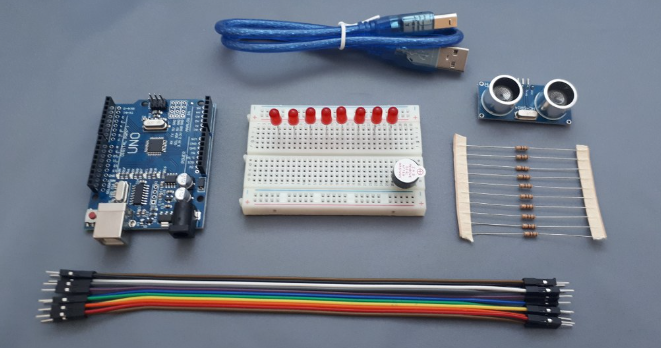
\includegraphics[width=0.73\textwidth]{Resimler/4.png}
\caption{Proje Malzemeleri Örneği}
\label{fig:4}
\end{figure}
\subsection{Kullanılan Malzemeler}
\begin{itemize}
    \item 1 Adet Breadboard
    \item Dişi- Erkek veya Erkek- Erkek Jumper Kablolar
    \item 1 Adet 220 Ohm Direnç
    \item 1 Adet HC-SR04 Arduino Ultrasonik Mesafe Sensörü
    \item 1 Adet Buzzer
    \item 1 Adet 2*16 Karakter LCD- I2C Modüllü Ekran
    \item 1 Adet RPM Redüktörlü DC Motor
    \item 1 Adet SG90 Mini Servo Motor
    \item 1 Adet L298N Motor Sürücü Kartı
    \item 1 Adet 9V Pil
    \end{itemize}

\subsection{Sistem Yazılımı}
    Sistem yazılımı Arduino IDE kullanılarak geliştirilmiştir. Bu yazılım, mesafeyi algılayarak aracı otomatik olarak park edebilen ve LCD ekranda bilgiler sunan bir düzenek için hazırlanmıştır. Yazılım, sensör verilerinin işlenmesi, servo motorun kontrolü ve uyarı sistemleri gibi çeşitli işlevleri entegre eder. Kodun detayları aşağıda verilmiştir. Genel olarak sistemin yazılım mantığı şu adımlardan oluşur:
    \begin{itemize}
        \item Mesafe sensörü ile engel algılanır.
        \item Mesafe bilgisi LCD’de görüntülenir.
        \item Servo motor ve buzzer ile uygun tepkiler verilir.
        \item Araç park edildikten sonra normal duruma geri dönülür.
    \end{itemize}
    
\subsubsection{Sensör ölçümleri}
    Ultrasonik sensör (HC-SR04) kullanılarak mesafe algılama işlemi yapılmaktadır. Sensörden gönderilen "trigger" sinyali yankı "echo" pini tarafından algılanır. Mesafe aşağıdaki formül ile hesaplanır:

    Bu hesaplama, şekil \ref{fig:31}'de olduğu gibi sesin havadaki yayılma hızı ve Arduino’daki \textbf{pulseIn()} fonksiyonu kullanılarak gerçekleştirilir.

\begin{figure}[H]
\centering
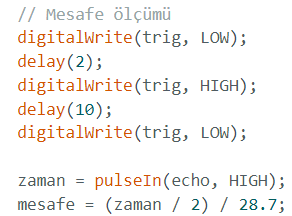
\includegraphics[width=0.40\textwidth]{Resimler/31.png}
\caption{Proje Mesafe Sensörü Kodu}
\label{fig:31}
\end{figure}

\subsubsection{LCD-I2C ekran kullanımı}
    I2C LCD modülü (0x27 adresi) kullanılarak, park sistemine ait bilgiler 16x2 LCD ekranda görüntülenir. Şekil \ref{fig:25}'de olduğu gibi ilk açılışta sistemin adı ve durumu ekrana yazılır. Çalışma sırasında mesafe bilgisi dinamik olarak ekranda gösterilir.
\begin{figure}[H]
\centering
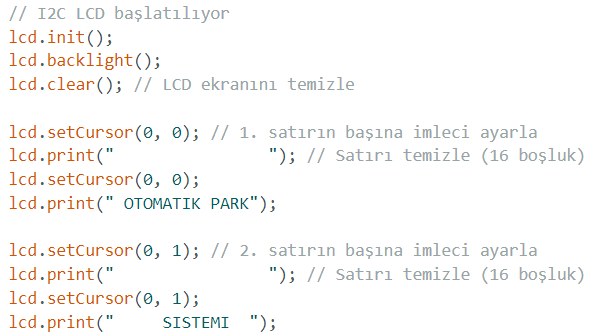
\includegraphics[width=0.85\textwidth]{Resimler/25.png}
\caption{Proje Lcd Kodu}
\label{fig:25}
\end{figure}
\subsubsection{Buzzer kullanımı}
    Buzzer, şekil \ref{fig:26}'de olduğu gibi mesafeye bağlı olarak farklı frekanslarda ses çıkartarak sürücüye uyarı verir. Mesafeye göre uyarı frekansları aşağıdaki gibidir:
\begin{itemize}
    \item \textbf{\underline{5 cm veya daha yakın:}} 1000 Hz (Hızlı uyarı)
    \item \textbf{\underline{5-10 cm:}} 800 Hz (Orta uyarı)
    \item \textbf{\underline{10-15 cm :}} 600 Hz (Yavaş uyarı)
    \item \textbf{\underline{15 cm veya daha uzak:}} Buzzer kapatılır
\end{itemize}

\begin{figure}[H]
\centering
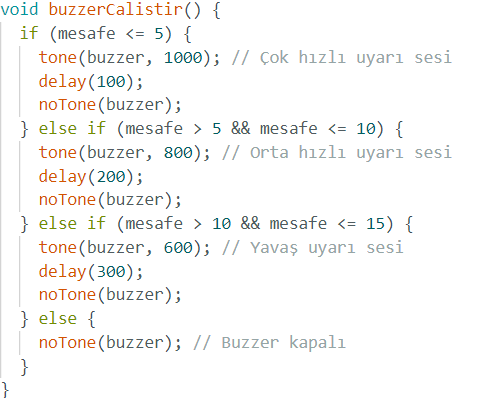
\includegraphics[width=0.50\textwidth]{Resimler/26.png}
\caption{Proje Buzzer Kodu}
\label{fig:26}
\end{figure}

\subsubsection{Servo motor kullanımı}
    Servo motor, park sırasında aracın tekerleklerini kontrol etmek için kullanılmaktadır. Şekil \ref{fig:27}'de olduğu gibi motor pozisyonları kontrol edilir:
\begin{itemize}
    \item \textbf{\underline{0 Derece:}} Park için sol hareket
    \item \textbf{\underline{180 Derece:}} Park için sağ hareket
    \item \textbf{\underline{90 Derece: }} Düz pozisyon
\end{itemize}

\begin{figure}[H]
\centering
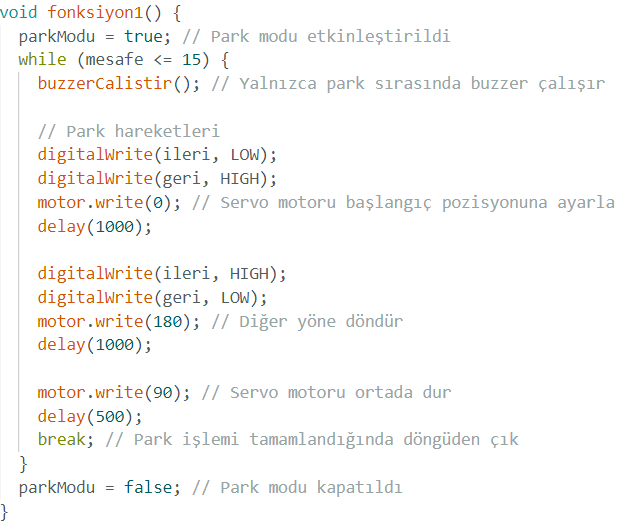
\includegraphics[width=0.55\textwidth]{Resimler/27.png}
\caption{Proje Servo Motor Kodu}
\label{fig:27}
\end{figure}

\subsubsection{Proje kodu}
Bütün proje kodu aşağıda gösterilmektedir:



\#include <Servo.h>\\
\#include <Wire.h>\\
\#include <LiquidCrystal\_I2C.h>

Servo motor;

int ileri = 2;\\
int geri = 3;\\
int trig = 8;\\
int echo = 9;\\
int buzzer = 13;

int zaman;\\
float mesafe;\\
bool parkModu = false; // Park modunu takip etmek için durum değişkeni

LiquidCrystal\_I2C lcd(0x27, 16, 2);\\
// I2C LCD için adres tanımı: Genelde 0x27 veya 0x3F kullanılır.

void buzzerCalistir()\\ 
\{\\
    if (mesafe <= 5)\\
    \{\\
    tone(buzzer, 1000); // Çok hızlı uyarı sesi\\
    delay(500);\\
    noTone(buzzer);\\
    \}\\
    else if (mesafe > 5 \&\& mesafe <= 10)\\
    \{\\
    tone(buzzer, 800); // Orta hızlı uyarı sesi\\
    delay(1000);\\
    noTone(buzzer);\\
    \}\\ 
    else if (mesafe > 10 \&\& mesafe <= 15)\\ 
    \{\\
    tone(buzzer, 600); // Yavaş uyarı sesi\\
    delay(1500);\\
    noTone(buzzer);\\
    \}\\ 
    else\\ 
    \{noTone(buzzer); // Buzzer kapalı\}\\
\}

void fonksiyon1()\\
\{\\
  parkModu = true; // Park modu etkinleştirildi\\
  while (mesafe <= 15)\\
  \{\\
    buzzerCalistir(); // Yalnızca park sırasında buzzer çalışır

    // Park hareketleri\\
    digitalWrite(ileri, LOW);\\
    digitalWrite(geri, HIGH);\\
    motor.write(0); // Servo motoru başlangıç pozisyonuna ayarla\\
    delay(1000);

    digitalWrite(ileri, HIGH);\\
    digitalWrite(geri, LOW);\\
    motor.write(180); // Diğer yöne döndür\\
    delay(1000);

    motor.write(90); // Servo motoru ortada dur\\
    delay(500);\\
    break; // Park işlemi tamamlandığında döngüden çık\\
  \}\\
  parkModu = false; // Park modu kapatıldı\\
\}

void setup()\\
\{\\
  delay(10000);

  Serial.begin(9600);\\
  motor.attach(6);

  pinMode(ileri, OUTPUT);\\
  pinMode(geri, OUTPUT);\\
  pinMode(trig, OUTPUT);\\
  pinMode(echo, INPUT);\\
  pinMode(buzzer, OUTPUT);

  Wire.begin();\\
  // I2C LCD başlatılıyor\\
  lcd.init();\\
  lcd.backlight();\\
  lcd.clear(); // LCD ekranını temizle

  lcd.setCursor(0, 0); // 1. satırın başına imleci ayarla\\
  lcd.print(" OTOMATIK PARK");\\
  lcd.setCursor(0, 1); // 2. satırın başına imleci ayarla\\
  lcd.print("     SISTEMI  ");\\
\}

void loop()\\
\{\\
  // Mesafe ölçümü\\
  digitalWrite(trig, LOW);\\
  delay(2);\\
  digitalWrite(trig, HIGH);\\
  delay(10);\\
  digitalWrite(trig, LOW);

  zaman = pulseIn(echo, HIGH);\\
  mesafe = (zaman / 2) / 28.7;


  if (!parkModu \&\& mesafe <= 15)\\
  \{\\
    // Park modu etkin değil ve mesafe uygunsa park etme fonksiyonunu çağır\\
    fonksiyon1();\\
    lcd.clear();\\
    lcd.setCursor(0, 0);\\
    lcd.print("  MESAFE: ");\\
    lcd.print(mesafe);\\
    lcd.print(" CM");\\
  \}\\
  else if (!parkModu)\\ 
  \{\\
    // Park modu aktif değilken araç düz hareket eder\\
    motor.write(90);\\
    digitalWrite(ileri, HIGH);\\
    digitalWrite(geri, LOW);
   
  \}

  delay(100);\\
\}

\subsection{Sistem Simülasyonu}
    Sistemin simülasyonu, Tinkercad platformu kullanılarak gerçekleştirilmiştir. Tinkercad, Arduino projelerini test etmek ve görsel olarak simüle etmek için kullanışlı bir çevrim içi aracıdır. Bu platform sayesinde, projeye ait devre tasarımı ve yazılım işlemleri sanal ortamda denenmiş ve optimize edilmiştir.

    Şekil \ref{fig:24}'de olduğu gibi simülasyonda, ultrasonik sensör, servo motor, buzzer ve LCD ekran gibi bütün bileşenlerin birbiriyle uyumlu bir şekilde çalıştığı test edilmiştir. Sistemin algoritması, platformdaki sanal çıktılar üzerinden doğrulanmış ve gerekli düzeltmeler yapılmıştır.

\begin{figure}[H]
\centering
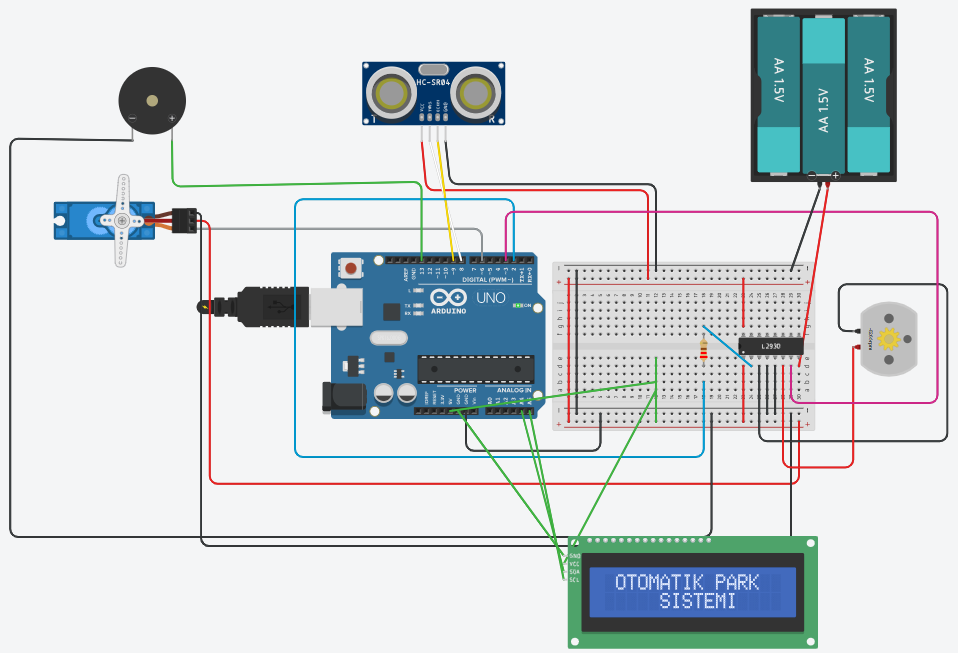
\includegraphics[width=0.85\textwidth]{Resimler/24.png}
\caption{Proje Simülasyonu}
\label{fig:24}
\end{figure}

\subsection{Araba Tasarımı}
    Bu projede, otomatik park sistemini desteklemek amacıyla bir prototip araba tasarlanmıştır. Şekil \ref{fig:32}, \ref{fig:33},  \ref{fig:34} ve \ref{fig:35}'da olduğu gibi tasarım tamamen el yapımı olup, gerekli tüm bileşenler dikkatlice monte edilmiştir. Arabanın altyapısı, Arduino tabanlı sensörler, servo motorlar, buzzer ve LCD ekran gibi elektronik bileşenleri taşımak üzere tasarlanmıştır. Tekerlekler ve gövde, hafif ve dayanıklı malzemelerden oluşturulmuş, elektronik devrelerin güvenli bir şekilde çalışmasını sağlayacak şekilde optimize edilmiştir.

\begin{figure}[H]
\centering
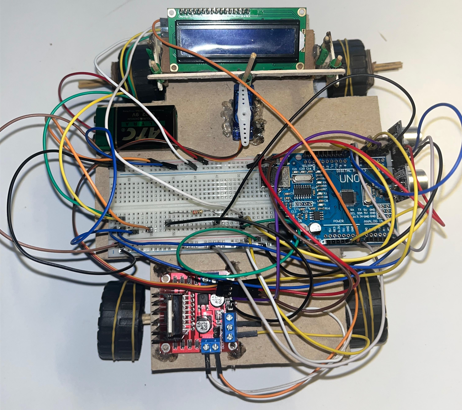
\includegraphics[width=0.75\textwidth]{Resimler/32.png}
\caption{Araba Tasarımı - 1 }
\label{fig:32}
\end{figure}

\begin{figure}[H]
\centering
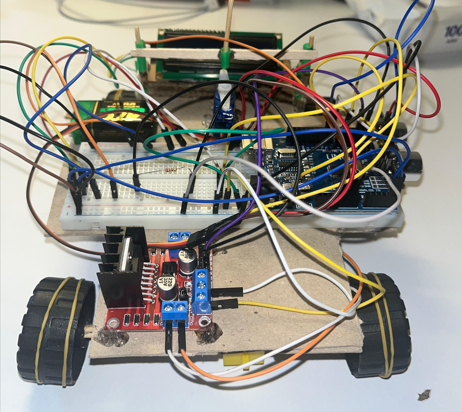
\includegraphics[width=0.70\textwidth]{Resimler/33.png}
\caption{Araba Tasarımı - 2 }
\label{fig:33}
\end{figure}

\begin{figure}[H]
\centering
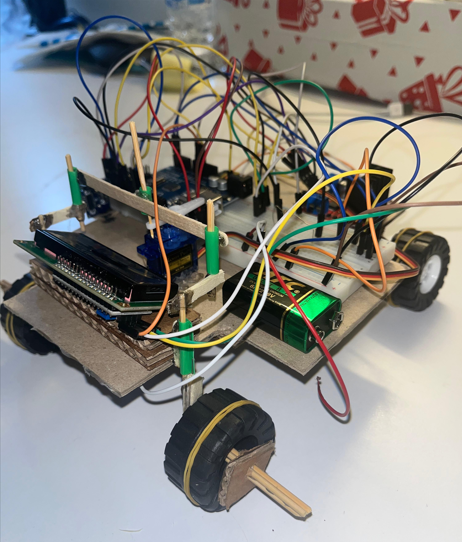
\includegraphics[width=0.65\textwidth]{Resimler/34.png}
\caption{Araba Tasarımı - 3 }
\label{fig:34}
\end{figure}

\begin{figure}[H]
\centering
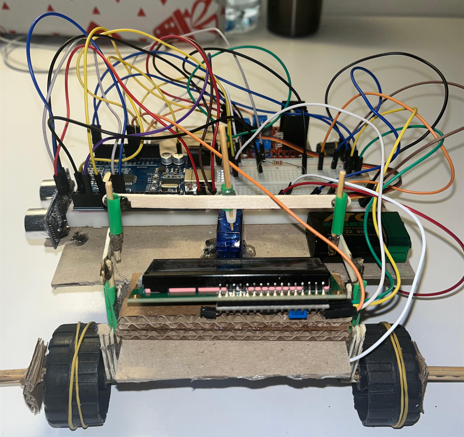
\includegraphics[width=0.65\textwidth]{Resimler/35.png}
\caption{Araba Tasarımı - 4 }
\label{fig:35}
\end{figure}
